\documentclass[11pt]{article}
\usepackage[margin=1in]{geometry}
\usepackage{amsmath,mathtools}
\usepackage{fancyhdr}
\usepackage{fancyvrb}
\usepackage{graphicx}
\usepackage{float}
\usepackage{color}
\usepackage{listings}
\pagestyle{fancy}
\fancyhead{}
\fancyfoot{}
\fancyhead[L]{{Project}}
\fancyfoot[C]{\thepage}
\definecolor{gray}{rgb}{0.95,0.95,0.95}
\lstset{
backgroundcolor=\color{gray}}
\begin{document}
\begin{titlepage}
\begin{center}
\vspace*{1cm}
\Large{\textbf{Monte Carlo Simulation}}\\
\Large{\textbf{(MA226)}}
\vfill
\line(1,0){500}\\[1mm]
\Huge{\textbf{Project}}\\[3mm]
\Large{\textbf{A convenient way to generate Gamma Random variables using generalized Exponential Distribution}}\\[1mm]
\line(1,0){500}\\
\vfill
By \\Mohammed Bilal Girach\\
Kodi Digvijay Yadav\\
Mamilla Rajasekhar\\
M.S.K.Prateek\\
G.Sai Vardhan Reddy\\
\vspace{1cm}
Supervised by\\
Arabin Kumar Dey\\
\today
\vfill
\end{center}
\end{titlepage}
\tableofcontents
\thispagestyle{empty}
\cleardoublepage
\setcounter{page}{1}
There are algorithms for shape parameter$(\alpha)<1$ and shape parameter$(\alpha)>1$.In this project we cite the methods for the case $0<\alpha <1$ and scale parameter $\lambda=1$\\
\ Two most popular methods are \\
\ $1.$Ahrens and  Dieter(AD)\\
\ $2.$Best\\
\section{Ahrens and  Dieter(AD)}
\  This method is based on the acceptance-rejection method with proper choice of majorization functions\\
\ Following is the majorization function\\ 

\[
t_{AD}(x;\alpha)=
\begin{dcases}
\frac{x^{\alpha-1}}{\Gamma(\alpha)}, & 0<x<1 \\
\frac{e^{-x}}{\Gamma(\alpha)}, & x>1
\end{dcases}
\]
$c_{AD}=\int_0^\infty t_{AD}(x;\alpha)\,\mathrm{d}x=\frac{(e+\alpha)}{e\Gamma(\alpha+1)}$\\
Now  we define a probability density function $r_{AD}$ which is obtained by dividing $c_{AD}$ with $\int_0^\infty t_{AD}(x;\alpha)\,\mathrm{d}x$\\
$$r_{AD}=\frac{t_{AD}}{\int_0^\infty t_{AD}(x;\alpha)\,\mathrm{d}x}$$\\
\[
r_{AD}(x;\alpha)=
\begin{dcases}
\frac{e\alpha x^{\alpha-1}}{e+\alpha}, & 0<x<1 \\
\frac{e\alpha e^{-x}}{e+\alpha}, & x>1
\end{dcases}
\]
\ The Cumulative Distribution Function of $r_{AD}$ is\\
\[
R_{AD}(x;\alpha)=
\begin{dcases}
\frac{e x^{\alpha}}{e+\alpha}, & 0<x<1 \\
1-\frac{\alpha e^{1-x}}{e+\alpha}, & x>1
\end{dcases}
\]
\ Gamma random variable for $\lambda=1$ and also $0<\alpha<1$\\

$$f_{GA}(x;\alpha)=
\frac{e^{- x}( x)^{(\alpha-1)}}{\Gamma(\alpha)};x>0$$ \\

\ \Large Supremum of $\frac{f_{GA}(x;\alpha)}{r_{AD}(x;\alpha)}=c_{AD}$. Proof is as follows\\
\[
\frac{f_{GA}(x;\alpha)}{r_{AD}(x;\alpha)}=
\begin{dcases}
\frac{e+\alpha}{e\Gamma(\alpha+1)e^{x}}\leq \frac{e+\alpha}{e\Gamma(\alpha+1)}=c_{AD},&0<x<1\\
\frac{(e+\alpha)x^{\alpha-1}}{e\Gamma(\alpha+1)}\leq  \frac{e+\alpha}{e\Gamma(\alpha+1)}=c_{AD},& x>1
\end{dcases}
\]
\subsection{Pseudo Code}
\begin{itemize}
\item Generate a uniform random number $U$
\item If $U\leq\frac{e}{e+\alpha}$ then $X=\left(U\left(\frac{e+\alpha}{e\alpha}\right)^{1/\alpha}\right)$ otherwise $X=-log(\frac{e+\alpha}{e\alpha}(1-U))$
\item Generate a uniform random number $V$;if $X\leq 1$  and if $V\leq e^{-X}$ then accept $X$ otherwise goto 1.If $X>1$ and if $V\leq X^{\alpha-1}$ then accept$X$ otherwise go back 1
\end{itemize}
\subsection{Code}
\lstinputlisting[language=R,frame = single]{AD.R}
\subsection{Sample graph}
For n=1000;$\alpha=0.9$
\begin{figure}[H]
\centering
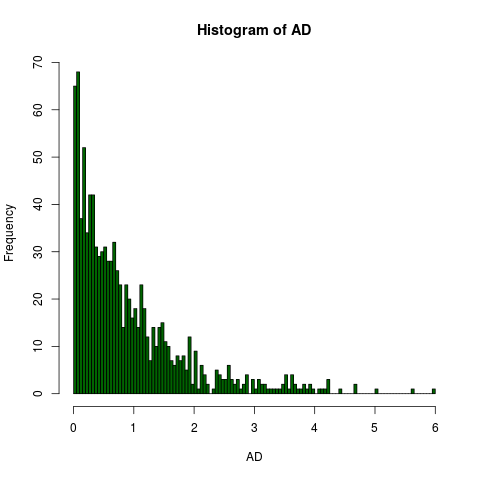
\includegraphics[scale=.65]{image1}
\end{figure}
\subsection{Output}
\begin{itemize}
\item Theoritical Acceptance via AD method: 0.7225393 
\item Acceptance Obtained: 0.7267442 
\end{itemize}
\section{Best}
\ Best used the following majorization function\\
\[
t_{B}(x;\alpha)=
\begin{dcases}
\frac{e x^{\alpha-1}}{\Gamma(\alpha)}, & 0<x<d \\
\frac{d^{\alpha-1e^{-x}}}{\Gamma(\alpha)}, & x>d
\end{dcases}
\]
\ $\int_0^\infty t_{B}(x;\alpha)\,\mathrm{d}x=\frac{d^{\alpha}}{\Gamma(\alpha)}\left[\frac{1}{\alpha}+e^{-d}\right]$\\
\ Choose d such that $\frac{d^{\alpha}}{\Gamma(\alpha)}\left[\frac{1}{\alpha}+e^{-d}\right]$ is minimum.It gives $$d=e^{-d}(1+\alpha-d)$$\\
\ The approximation for d given by Best is\\
\ $$d=0.07+0.75\sqrt{1-\alpha}$$
Now  we define a probability density function $r_{AD}$ which is obtained by dividing $r_{B}$ with $\int_0^\infty t_{B}(x;\alpha)\,\mathrm{d}x$
\[
r_{B}(x;\alpha)=
\begin{dcases}
\frac{\alpha e x^{\alpha-1}}{bd^{\alpha}}, & 0<x<d \\
\frac{\alpha e^{-x}}{bd}, & x>d
\end{dcases}
\]
\ where $b=1+\frac{\alpha e^{-d}}{d}$\\$c_{B}$=supremum of $\frac{f_{GA}(x,\alpha)}{r_{B}(x,\alpha)}$=$\frac{(d+\alpha e^{-d})d^{\alpha-1}}{\Gamma(\alpha+1)}$\\\\
The Cumulative Distribution Function of $r_{AD}$ is\\
\[
R_{B}(x;\alpha)=
\begin{dcases}
\frac{1}{b}\left(\frac{x}{d}\right)^{\alpha}, & 0<x<d \\
\frac{1}{b}+\frac{a(e^{-d}-e^{-x})}{bd}, & x>d
\end{dcases}
\]
\ Gamma random variable for $\lambda=1$ and also $0<\alpha<1$\\

$$f_{GA}(x;\alpha)=
\frac{e^{- x}( x)^{(\alpha-1)}}{\Gamma(\alpha)};x>0$$ \\
\subsection{Pseudo code}
\begin{itemize}
\item Generate a uniform random number $U$
\item If $U\leq\frac{1}{b}$ then $X=d(bU)^{1/\alpha}$ otherwise $X=-log(e^{-d}+(\frac{1}{b}-U)\frac{bd}{\alpha})$
\item Generate a uniform random number $V$;if $X\leq 1$  and if $V\leq e^{-X}$ then accept $X$ otherwise goto 1.If $X>1$ and if $V\leq \left(\frac{X}{d}\right)^{\alpha-1}$ then accept$X$ otherwise go back 1
\end{itemize}
\subsection{Code}
\lstinputlisting[language=R,frame = single]{Best.R}
\subsection{Sample graph}
For n=1000;$\alpha=0.9$
\begin{figure}[H]
\centering
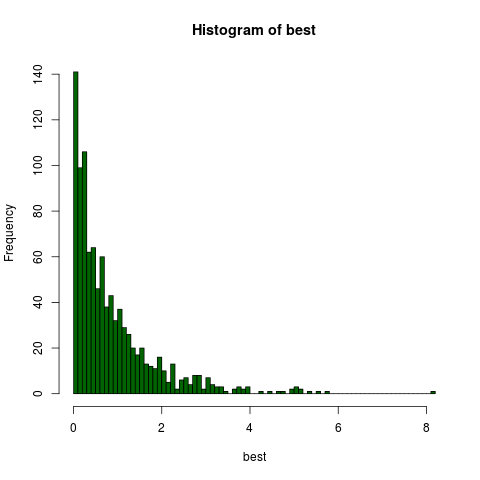
\includegraphics[scale=.65]{image2}
\end{figure}
\subsection{Output}
\begin{itemize}
\item Theoritical Acceptance via Best method: 0.8819001 
\item Acceptance Obtained: 0.8710801
\end{itemize}
\section{Proposed Methology}
In this section, we provide the new gamma random number generator using the generalized exponential distribution.
\begin{flushleft}
\textbf{Generalized exponential distribution}
\end{flushleft}
\[
f_{GE}(x;\alpha)=
\begin{dcases}
\ 0 & x<0 \\
\ \alpha\lambda(1-e^{-\lambda x})^{\alpha-1}, & x>0
\end{dcases}
\]
\ Gamma random variable for $\lambda=1$ and also $0<\alpha<1$\\
$$f_{GA}(x;\alpha)=
\frac{e^{- x}( x)^{(\alpha-1)}}{\Gamma(\alpha)};x>0$$ \\
\subsection{Algorithm 1}
In this Algorithm we choose Generalized exponential density function $f_{GE}(x;\alpha;\frac{1}{2})$ to be our majorization function.\\
\begin{center}
\ \textbf{Supremum} of $\frac{f_{GA}}{f_{GE}(x;\alpha;\frac{1}{2})}=\frac{2^{\alpha}}{\Gamma(\alpha+1)}$
\end{center}
\subsubsection{Psuedo Code}
\begin{itemize}
\item Generate U from uniform (0,1).
\item Compute $X = -2\ln\left(1-U^{\frac{1}{\alpha}}\right).$
\item Generate V from uniform (0,1) independent of U.
\item if $V \leq \frac{X^{\alpha-1}e^{-X/2}}{2^{\alpha-1}\left(1-e^{-X/2}\right)^{\alpha-1}}$ accept X, otherwise goto beginning.
\end{itemize}
\subsubsection{Code}
\lstinputlisting[language=R,frame = single]{algo1.R}
\subsubsection{Sample graph}
For n=1000;$\alpha=0.9$
\begin{figure}[H]
\centering
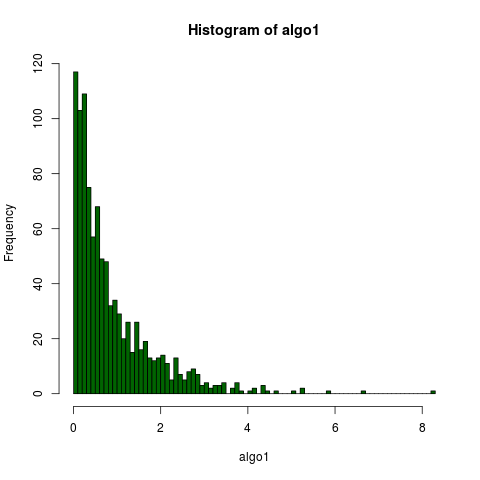
\includegraphics[scale=.65]{image3}
\end{figure}
\subsubsection{Output}
\begin{itemize}
\item Theoritical acceptance via alg1: 0.5153976 
\item Acceptance Obtained: 0.5216484 
\end{itemize}
\subsection{Algorithm 2}
The bound proposed is sharp for $0<x<1$,but for $1<x<\infty$ the bound is\\
not very sharp.So the following majorization function $t_{1}(x,\alpha)$ of      $f_{GA}(x,\alpha)$  is proposed i.e, $\forall$ $x>0$ $f_{GA}(x,\alpha)\leq t_{1}(x,\alpha)$\\ \\
It is observed that multiplication of  GE function by  a constant can be used as a majorization function in the interval $(0<x<1)$.The constant used is c.We propose the following \textbf{majorization} function:\\
We propose the following \textbf{majorization} function:
\[
t_1(x;\alpha) = 
\begin{dcases}
\frac{2^{\alpha}}{\Gamma(\alpha+1)}f_{GE}(x;\alpha,\frac{1}{2}), & 0<x<1\\
\frac{1}{\Gamma(\alpha)}e^{-x}, & x>1 
\end{dcases}
\]
$c_1=\int_0^\infty
t_1(x;\alpha)\,\mathrm{d}x=\frac{1}{\Gamma(\alpha+1)}\left[2^{\alpha}\left(1-e^{\frac{-1}{2}}\right)^{\alpha}+\alpha e^{-1}\right]$\\ \\
Now we define a probability density fumction $r_1$ which is obtained by dividing $t_1(x;\alpha)$ with $c_1$:
$$r_1(x;\alpha) = \frac{1}{c_1}t_1(x;\alpha);     x>0$$\\
which has the following distribution function:
\[
R_1(x;\alpha)=
\begin{dcases}
0, & x<0\\
\frac{2^\alpha}{c_1 \Gamma(\alpha+1)}\left(1-e^{\frac{-x}{2}}\right)^{\alpha}, & 0<x<1\\
1-\frac{1}{c_1 \Gamma(\alpha)}e^{-x}, & x>1\\
\end{dcases}
\]
\subsubsection{Pseudo Code}
Set $a = \frac{\left(1-e^{-1/2}\right)^{\alpha}}{\left(1-e^{-1/2}\right)^{\alpha}+\frac{\alpha e^{-1}}{2^\alpha}}$ and $b = \left(1-e^{-1/2}\right) + \frac{\alpha e^{-1}}{2^\alpha}$
\begin{itemize}
\item Generate U from uniform (0,1).
\item If U $\leq$ $X = -2\ln\left[1-(Ub)^{\frac{1}{\alpha}}\right]$, otherwise $X = -\ln\left[\frac{2^\alpha}{\alpha}b(1-U)\right]$.
\item Generate V from uniform (0,1) independent of U. If X $\leq$ 1, check whether $V \leq \frac{X^{\alpha-1}e^{-X/2}}{2^{\alpha-1}\left(1-e^{-X/2}\right)^{\alpha-1}}.$ If true return X, otherwise bo back to the beginning. If X $>$ 1, check whether V $\leq$ $X^{\alpha-1}$. If true return X, otherwise go back to the beginning.
\end{itemize}
\subsubsection{Code}
\lstinputlisting[language=R,frame = single]{algo2.R}
\subsubsection{Sample graph}
For n=1000;$\alpha=0.9$
\begin{figure}[H]
\centering
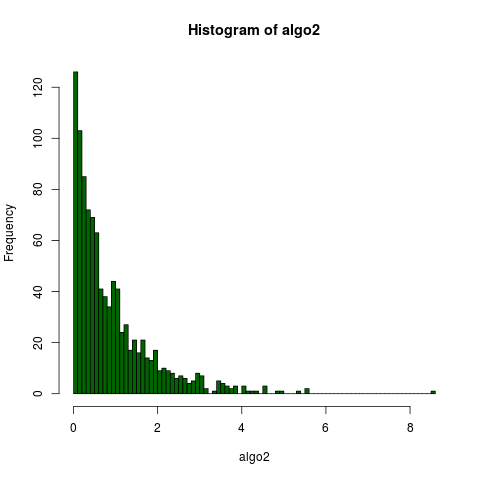
\includegraphics[scale=.65]{image4}
\end{figure}
\subsubsection{Output}
\begin{itemize}
\item Theoritical Acceptance via alg2: 0.845796 
\item Acceptance Obtained 0.8591065  
\end{itemize}
\subsection{Algorithm 3}
Now we propose the following modified majorization function:
\[
t_2(x;\alpha)=
\begin{dcases}
\frac{2^{\alpha}}{\Gamma(\alpha+1)}f_{GE}(x,\alpha,\frac{1}{2}), & 0<x<d_\alpha\\
\frac{1}{\Gamma(\alpha)}d^{\alpha-1}_\alpha e^{-x}, & x>d_\alpha
\end{dcases}
\]
$c_2=\int_0^\infty
t_2(x;\alpha)\,\mathrm{d}x=\frac{1}{\Gamma(\alpha+1)}\left[2^{\alpha}\left(1-e^{\frac{-d_\alpha}{2}}\right)^{\alpha}+\alpha d^{\alpha-1}_\alpha e^{-d\alpha}\right]$\\ \\
We now generate the following distribution function:
\[
R_2(x;\alpha)=
\begin{dcases}
0, & x<0\\
\frac{2^\alpha}{c_2 \Gamma(\alpha+1)}\left(1-e^{\frac{-x}{2}}\right)^{\alpha}, & 0<x<d_\alpha\\
1-\frac{1}{c_2 \Gamma(\alpha)}d^{\alpha-1}_\alpha e^{-x}, & x>d_\alpha\\
\end{dcases}
\]
We denote the optimum choice of $d_\alpha$ as $d_\alpha^o$.\\
We suggest the following approximation of the optimum $d_\alpha^o$ as $d_\alpha^*$, where $$d_\alpha^* = 1.0334-0.0766e^{2.2942\alpha}$$\\
\subsubsection{Pseudo Code}
Set $d = 1.0334-0.0766e^{2.2942\alpha}$, $a = 2^\alpha\left(1-e^{\frac{-d}{2}}\right)^\alpha$, $b = \alpha d^{\alpha-1}e^{-d}$ and $c = a + b$.
\begin{itemize}
\item Generate U from uniform (0,1).
\item If U $\leq$ $\frac{a}{a+b}$, then $X = -2\ln\left[1-\frac{(cU)^{1/\alpha}}{2}\right]$, otherwise $X = -\ln\left[\frac{c(1-U)}{\alpha d^{\alpha-1}}\right]$.
\item Generate V from uniform (0,1). If X $\leq$ d, check whether $V \leq \frac{X^{\alpha-1}e^{-X/2}}{2^{\alpha-1}\left(1-e^{-X/2}\right)^{\alpha-1}}.$ If true return X, otherwise bo back to the beginning. If X $>$ d, check whether V $\leq$ $\left(\frac{d}{X}\right)^{1-\alpha}$. If true return X, otherwise go back to the beginning.
\end{itemize}
\subsubsection{Code}
\lstinputlisting[language=R,frame = single]{algo3.R}
\subsubsection{Sample graph}
For n=1000;$\alpha=0.9$
\begin{figure}[H]
\centering
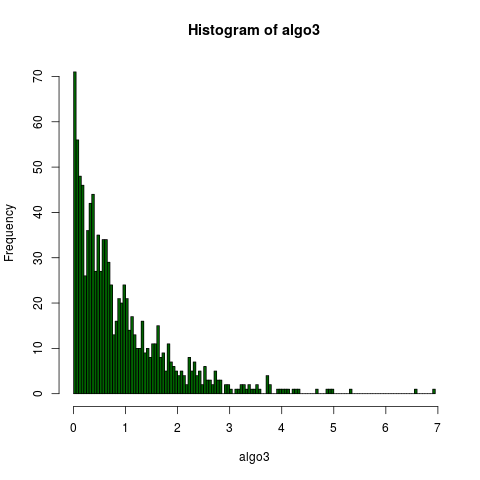
\includegraphics[scale=.65]{image5}
\end{figure}
\subsubsection{Output}
\begin{itemize}
\item Theoritical acceptance via alg3: 0.9052209 
\item Acceptance Obtained: 0.8976661   
\end{itemize}
\section{Analysis on different methods}
\subsection{Code}
\lstinputlisting[language=R,frame = single]{31.R}
\subsection{Tabulated Data}
\begin{center}\textbf{\underline{Acception Probability through various methods}} \end{center}
\begin{tabular}{|c|c|c|c|c|c|}
\hline
$\alpha$ & AD Method & Best Method & Algorithm1 & Algorithm2 & Algorithm3\\\hline 
0.1  & 0.9141603 & 0.9198786 & 0.8608815 & 0.9203019 & 0.9126586 \\ \hline
0.2  & 0.8514261 & 0.8586639 & 0.7924558 & 0.8945344 & 0.891504 \\ \hline
0.3  & 0.8082114 & 0.8230453 & 0.7248478 & 0.8644537 & 0.8719156 \\ \hline
0.4  & 0.7713074 & 0.7983395 & 0.6719527 & 0.8368901 & 0.8423181 \\ \hline
0.5  & 0.7475518 & 0.7786949 & 0.6282196 & 0.8290499 & 0.8385041 \\ \hline
0.6  & 0.7373544 & 0.7845599 & 0.5934366 & 0.8273352 & 0.8281573 \\ \hline
0.7  & 0.7184424 & 0.7994244 & 0.5560807 & 0.8211529 & 0.8386448 \\ \hline
0.8  & 0.7203573 & 0.8271983 & 0.5368839 & 0.8358409 & 0.8628128 \\ \hline
0.9  & 0.7251632 & 0.877809 & 0.5147475 & 0.8489685 & 0.903424 \\ \hline
\end{tabular}
\subsection{Graph}
For all methods
\begin{figure}[H]
\centering
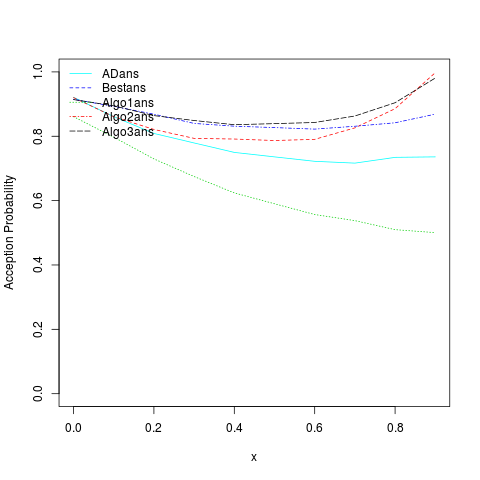
\includegraphics[scale=1]{Main}
\end{figure}
\end{document}
